\documentclass[12pt]{article}

%useful packages
\usepackage{color,soul}
\usepackage[usenames,dvipsnames,svgnames,table]{xcolor}
\usepackage{amsmath,amsthm,amscd,amssymb,bm}
\usepackage{hyperref}
\hypersetup{
    colorlinks=true,
    linkcolor=JungleGreen,
    urlcolor  =JungleGreen,
    citecolor = JungleGreen,
    anchorcolor = JungleGreen
}
\usepackage[utf8]{inputenc}
\usepackage[top=2cm, bottom=3cm, left=2cm, right=2cm]{geometry}
\usepackage{pgfplots}
\usepackage{enumitem}
\usepgfplotslibrary{fillbetween}
\usetikzlibrary{patterns}
\usepackage{tcolorbox}
\usepackage{centernot}
\usepackage{mathtools}
\usepackage{xcolor}
\usepackage{subcaption}

%personal definitions and commands
\newcommand{\R}{\mathbb{R}} 
\newcommand{\E}{\mathbb{E}}
\newcommand{\V}{\mathbb{V}}
\newcommand{\C}{\mathbb{C}}
\newcommand{\Prob}{\mathbb{P}}
\newcommand{\e}{\epsilon}
\newcommand\numberthis{\addtocounter{equation}{1}\tag{\theequation}} %allows numbering of single equations in align* environment
\newcommand{\mtx}[1]{\ensuremath{\bm{\mathit{#1}}}}
\newcommand{\B}{\hat{\boldsymbol{\beta}}}
\newcommand{\Cov}{\mathbb{C}\text{ov}}
\newcommand{\N}{\mathcal{N}}



\title{ECON675 -- Assignment 6}
\author{Anirudh Yadav}
\setlength\parindent{0pt}
\begin{document}

\maketitle

\setcounter{tocdepth}{2}
\tableofcontents

\newpage

\section{The effect of Head Start on child mortality}

\subsection{RD plots and falsification tests}
\begin{figure}[htpb!]
    \centering
    \caption{RD Plots of Pre-intervention Mortality Rates Using Different Binning Procedures}
    \begin{minipage}{0.5\textwidth}
        %\centering
        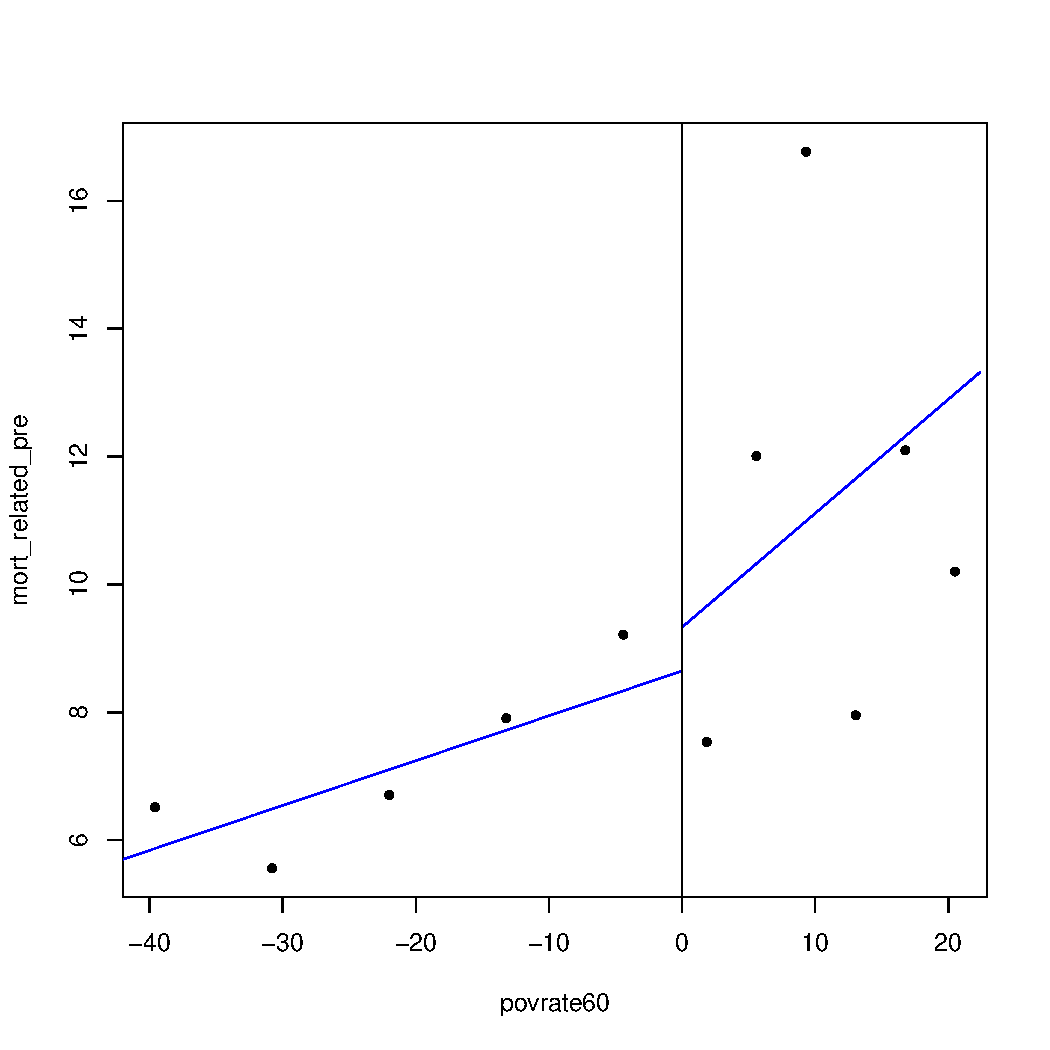
\includegraphics[width=1\textwidth]{q2-1-es.pdf}
        \subcaption{Evenly-spaced, IMSE optimal}
    \end{minipage}\hfill
    \begin{minipage}{0.5\textwidth}
      %  \centering
        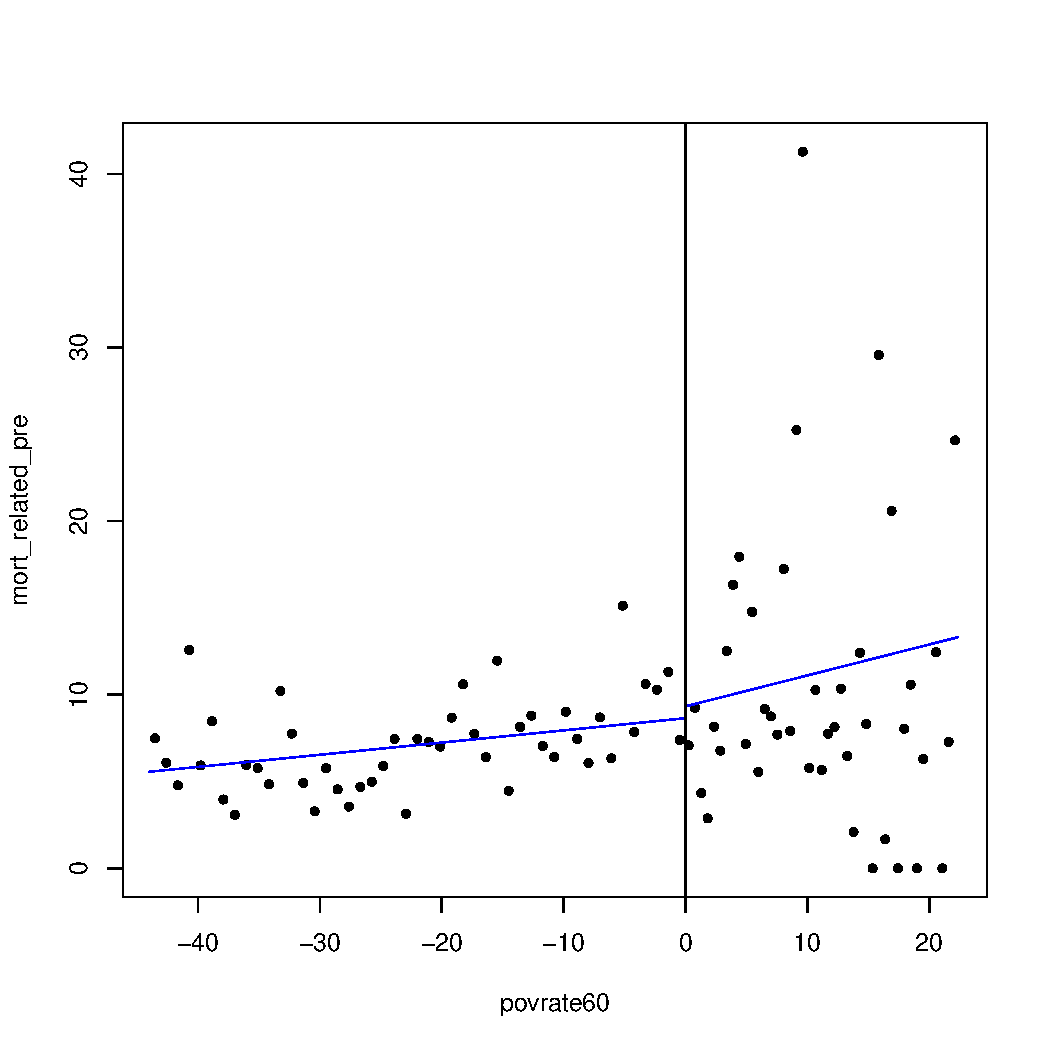
\includegraphics[width=1\textwidth]{q2-1-esmv.pdf}
        \subcaption{Evenly-spaced, variance mimicking}
    \end{minipage}
\centering
\begin{minipage}{0.5\textwidth}
        %\centering
        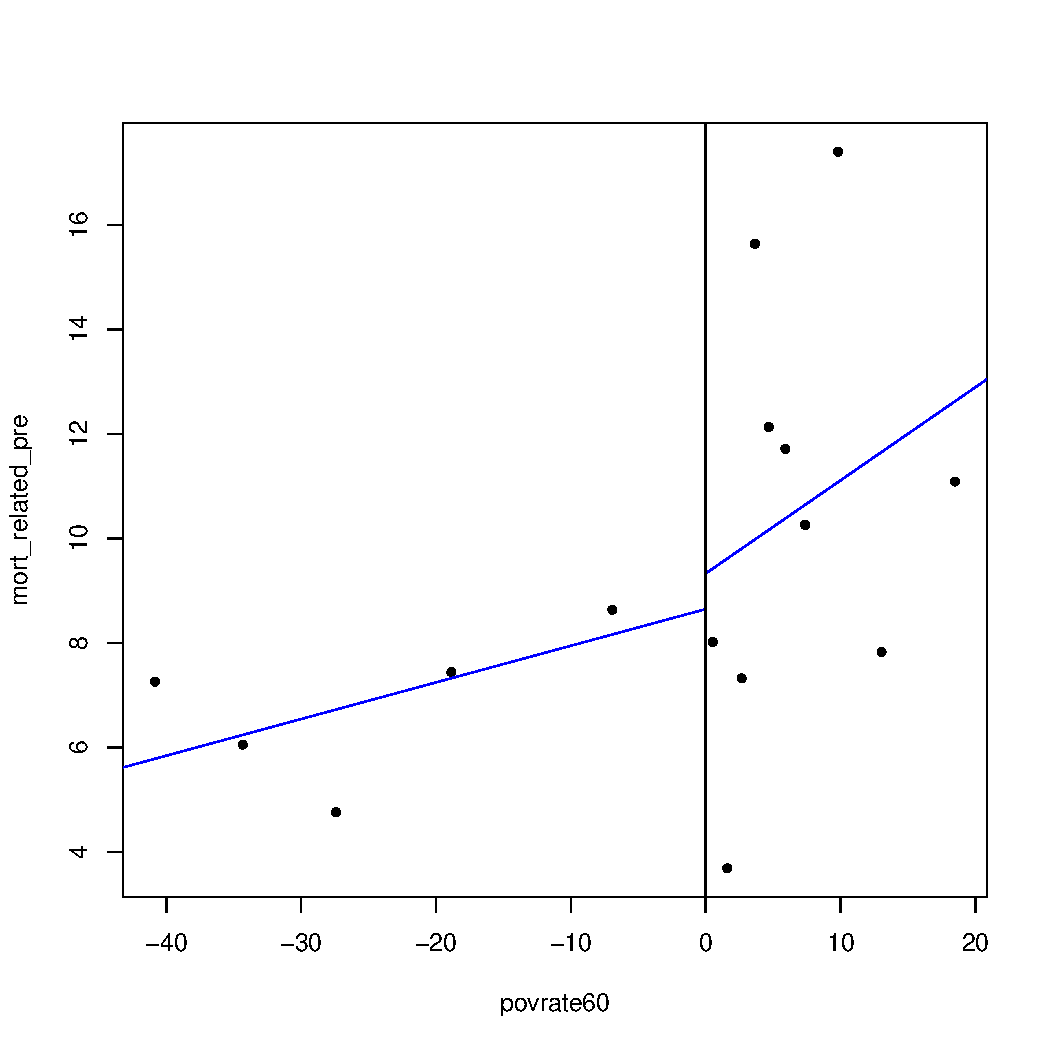
\includegraphics[width=1\textwidth]{q2-1-qs.pdf}
        \subcaption{Quantile-spaced, IMSE optimal}
    \end{minipage}\hfill
    \begin{minipage}{0.5\textwidth}
      %  \centering
        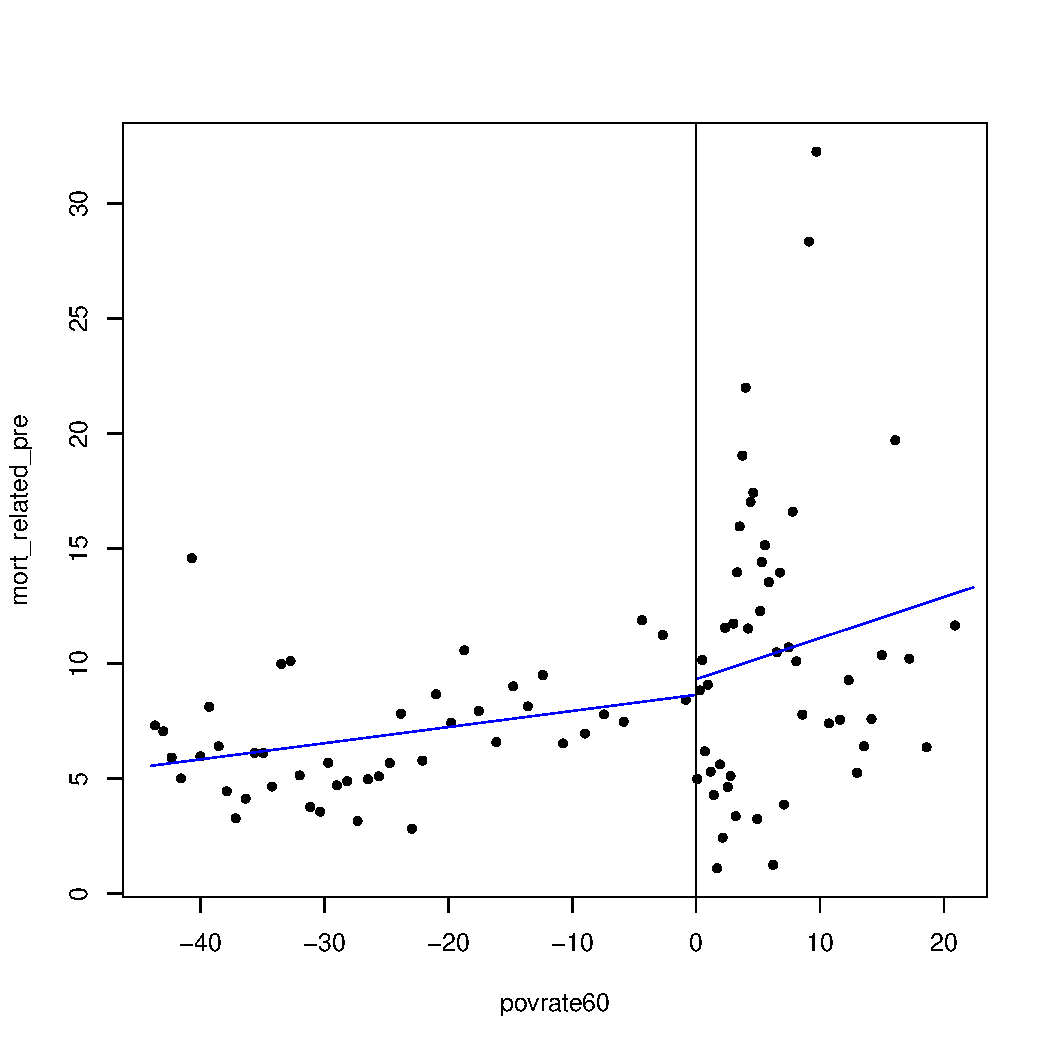
\includegraphics[width=1\textwidth]{q2-1-qsmv.pdf}
        \subcaption{Quantile-spaced, variance mimicking}
    \end{minipage}
\end{figure}

Figure 1 shows the RD plots of \verb|mort_related_pre| using different binning procedures, as required. For each binning method, there is clearly no evidence of a negative discontinuity at the cutoff poverty rate. (In fact, there seems to be a small positive jump in pre-invervention mortality rates at the cutoff.) If there was a negative jump in pre-intervention mortality rates at the cutoff this would potentially falsify the proposed RD design because it would provide strong evidence that the counties assigned to Head Start treatment had systematically lower mortality rates prior to the intervention.\\

We can also conduct formal falsification tests. First, I conduct exact binomial tests for small windows around the cutoff. The basic idea is that if there is no systematic sorting, then the number of observations just above or below the cutoff should be pretty close to random, and thus should follow a binomial distribution. Table 1 shows the results for the exact binomial test (with probability of success set to 0.5) for a few small windows near the cutoff (replicating Table 1 in Cattaneo, \textit{et al}. (2017)). Clearly, we cannot reject the null that the number of observations just above and below the cutoff are random.

\begin{table}[htpb!]
\centering
\caption{Binomial tests}
\begin{tabular}{llrrr}
  \hline
 & $h$ & $N_W^-$ & $N_W^+$ & $p$-value \\ 
  \hline
1 & 0.3 & 9 & 10 & 1.000 \\ 
  2 & 0.5 & 18 & 16 & 0.864 \\ 
  3 & 0.7 & 24 & 22 & 0.883 \\ 
  4 & 0.9 & 32 & 27 & 0.603 \\ 
  5 & 1.1 & 43 & 33 & 0.302 \\ 
  6 & 1.3 & 51 & 38 & 0.203 \\ 
   \hline
\end{tabular}
\end{table}

Next, I test for a discontinuity in the density of the running variable at the cutoff, as in Cattaneo, \textit{et al}. (2017), using the \verb|rddensity| package in \verb|R|. I compute the density test $p$-value using the package defaults, which specifies a local-quadratic polynomial estimator with triangular kernel and jackknife standard errors. I get $p = 0.639$, implying that we cannot reject the null that the density of the running variable is continuous at the cutoff.

\subsection{Global and flexible parametric methods}
I estimate the following global polynomial regression models
\begin{align*}
y_i = \alpha_0 + \beta_0 t_i + \sum_{k=1}^p \beta_k x_i^k + \e_i
\end{align*}
where $y_i$ is the outcome of interest (post-intervention mortality rate) and $x_i$ is the running variable (poverty rate in 1960) and $t_i$ is a treatment dummy equal to 1 if $x_i \geq 0$. Table 2 presents the point estimates of $\beta_0$ for $p=3,4,5,6$ and the corresponding robust standard errors. The estimated treatment effects are all negative as expected. \\

Despite the negative estimated treatment effects, these are bad models. They all use global methods, but we know that RD treatment effects are inherently local to the cutoff. In essence, global methods do not compare `apples with apples', because counties well below or above the cutoff could be different in systematically important ways.

\begin{table}[htpb!]
\centering
\caption{Global Polynomial Fit under Constant Treatment Effect Assumption}
\begin{tabular}{lrrrr}
  \hline
 & $p=3$ & $p=4$ & $p=5$ & $p=6$ \\ 
  \hline
Point estimate& $-1.12$ & $-1.02$ & $-1.66$ & $-1.75$ \\ 
Std. err. & 0.59 & 0.75 & 0.81 & 0.86 \\ 
   \hline
\end{tabular}
\end{table}

\subsection{Robust local polynomial methods}

\subsubsection{Baseline estimates}
Table 3 shows the MSE-optimal RD point estimators and robust confidence intervals using local constant, linear and quadratic estimators (implemented with the \verb|rdrobust| package in \verb|R|). The estimated treatment effects are negative and significantly different from zero for all specifications, as expected. The standard errors of the point estimates increase with the order of the local polynomial.

\begin{table}[htpb!]
\centering
\caption{MSE-Optimal RD Treatment Effects with Different Polynomial Estimators}
\begin{tabular}{lrrrr}
  \hline
 & Coeff & Std. Err. & CI Lower & CI Upper \\ 
  \hline
  \multicolumn{5}{c}{$p=0$}\\
  \hline
Conventional & -2.11 & 0.99 & -4.05 & -0.17 \\ 
  Bias-Corrected & -2.56 & 0.99 & -4.50 & -0.62 \\ 
  Robust & -2.56 & 1.23 & -4.96 & -0.15 \\ 
   \hline
   \multicolumn{5}{c}{$p=1$}\\
     \hline
Conventional & -2.41 & 1.21 & -4.77 & -0.05 \\ 
  Bias-Corrected & -2.78 & 1.21 & -5.14 & -0.42 \\ 
  Robust & -2.78 & 1.37 & -5.46 & -0.10 \\ 
   \hline
\multicolumn{5}{c}{$p=2$}\\
     \hline
Conventional & -3.47 & 1.37 & -6.16 & -0.79 \\ 
  Bias-Corrected & -3.78 & 1.37 & -6.46 & -1.10 \\ 
  Robust & -3.78 & 1.45 & -6.62 & -0.94 \\ 
   \hline
\end{tabular}
\end{table}

\subsubsection{Placebo tests}
Table 4 shows estimated RD treatment effects for the pre-intervention outcome variable \verb|mort_related_pre| and the unaffected post-intervention variable, \verb|mort_injury_post|. Clearly, we cannot reject the null of no treatment effect on these placebo outcomes.

\begin{table}[htpb!]
\centering
\caption{Robustness Checks of RD Treatment Effects using Different Outcome Variables}
\begin{tabular}{lrrrr}
  \hline
 & Coeff & Std. Err. & CI Lower & CI Upper \\ 
  \hline
  \multicolumn{5}{c}{$y= \texttt{mort\_related\_pre}$}\\
  \hline
Conventional & -2.38 & 2.25 & -6.78 & 2.03 \\ 
  Bias-Corrected & -1.77 & 2.25 & -6.17 & 2.64 \\ 
  Robust & -1.77 & 2.68 & -7.01 & 3.48 \\ 
   \hline
 \multicolumn{5}{c}{$y= \texttt{mort\_injury\_post}$}\\
     \hline
Conventional & 1.13 & 3.77 & -6.26 & 8.53 \\ 
  Bias-Corrected & 1.52 & 3.77 & -5.87 & 8.92 \\ 
  Robust & 1.52 & 4.39 & -7.07 & 10.12 \\
   \hline
\end{tabular}
\end{table}

\subsection{Local randomization inference}
I use the \verb|rdlocrand| package in \verb|R| to conduct local randomization inference on the Head Start data.

\subsubsection{Window selection}
First we need to select a window around the cutoff where randomization inference is appropriate. To do so, I use the \verb|rdwinselect| function in \verb|R|, with pre-intervention covariate \verb|mort_related_pre| and the unaffected post-intervention variable, \verb|mort_injury_post|. The basic idea is to choose the largest window around the cutoff where these covariates (which should not be related to the treatment) are ``reasonably'' balanced for counties above and below the cutoff. Essentially, we're trying to choose the biggest window around the cutoff where counties' poverty rates are pretty much random. Within this window, the RD design can be interpreted as a randomized experiment.\\

Using \verb|rdwinselect| (and the default options), the recommended window is $[-0.976;0.976]$ with 126 observations (68 below, 58 above).

\subsubsection{Randomization inference}
With the recommended window above, the observed difference in means is $-2.304\%$, with Fisher exact $p$-value of $0.024$ (associated with the sharp null of no treatment effect and 1000 replications).


\newpage


\section{Appendix: \texttt{R} code}




\end{document}
